
\section{Periodic Table of Storytelling }


\begin{center}
	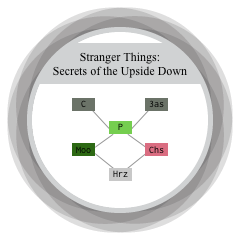
\includegraphics[width=0.75\linewidth]{images/story_molecolar.png}
\end{center}

\vspace*{2mm}

Description of the elements:\\
\textbf{\textcolor{LimeGreen}{[P]} Protagonist}: Bad Eleven is the protagonist of the story.\\
%\textbf{\textcolor{LimeGreen}{[A]} Antagonist}: Kyle, a powerful magician.\\
%\textbf{\textcolor{LimeGreen}{[Rnd]} Rounded Character​}: \#010 gradually loses her kind-hearted attitude during the story due to the death of her brother. In the end she will turn good again and feel guilty for the bad feelings harboring in her heart.\\
\textbf{\textcolor{dark-gray}{[3as]} Three Act Structure}: The story begins with a Setup act (introduction of characters setting and context), continues with a Confrontation and Evolution act (meeting with \#009 and \#010 encounters \#001) and ends with a Resolution act (after the final battle the protagonist ends his evolution).\\
%\textbf{\textcolor{dark-gray}{[Cmx]} The Climax}: The final battle is the most important event in the story, involving directly and indirectly every characters.\\
\textbf{\textcolor{dark-gray}{[C]} Conflict}: Kyle has a plan to control the Upside-Down Core and he kills \#005 and \#010 for this purpose. Elby will stop him with \#009 help, who is looking for revenge.\\
\textbf{\textcolor{OliveGreen}{[Moo]} Mooks}: The standard enemies, like Demonrats and Demondogs.\\
\textbf{\textcolor{Salmon}{[Chs]} The Chessmaster}: Kyle gets the name of chessmaster from his ability to manipulate events. he uses the protagonist to obtain informations about the numbers and uses them as if they were pieces on a chessboard.\\
\textbf{\textcolor{light-gray}{[Hrz]} Moral Event Horizon}: After the end of the Act II, Kyle'll have a mental breakdown and will become like a mindless man seeking only destruction. From that moment he will be pure evil.\\